\documentclass{jcgt}

\setciteauthor{Guanyu He and Hao Wu}
\setcitetitle{WebGL Ocean Simulation using Fast Fourier Transformation}

% Mark submissions with the date of submission using the following line:
\submitted{\today}

% Once an article is accepted accepted, switch to the following line and comment the preceding one. The editor will supply the argument values.
\accepted{July 4, 2013}{July 4, 2013}{July 4, 2013}{Editor Name}{2}{1}{1}{1}{2013}
\seturl{http://jcgt.org/published/0002/02/01/}




%%%%%%%%%%%%%%%%%%%%%%%%%%%%%%%%%%%%%%%%%%%%%%%%%%%%


\begin{document}

\title{WebGL Ocean Simulation using Fast Fourier Transformation}

\author
       {Guanyu He\\University of Pennsylvania
        \and Hao Wu\\University of Pennsylvania
       }

% Optional teaser image
\teaser{
  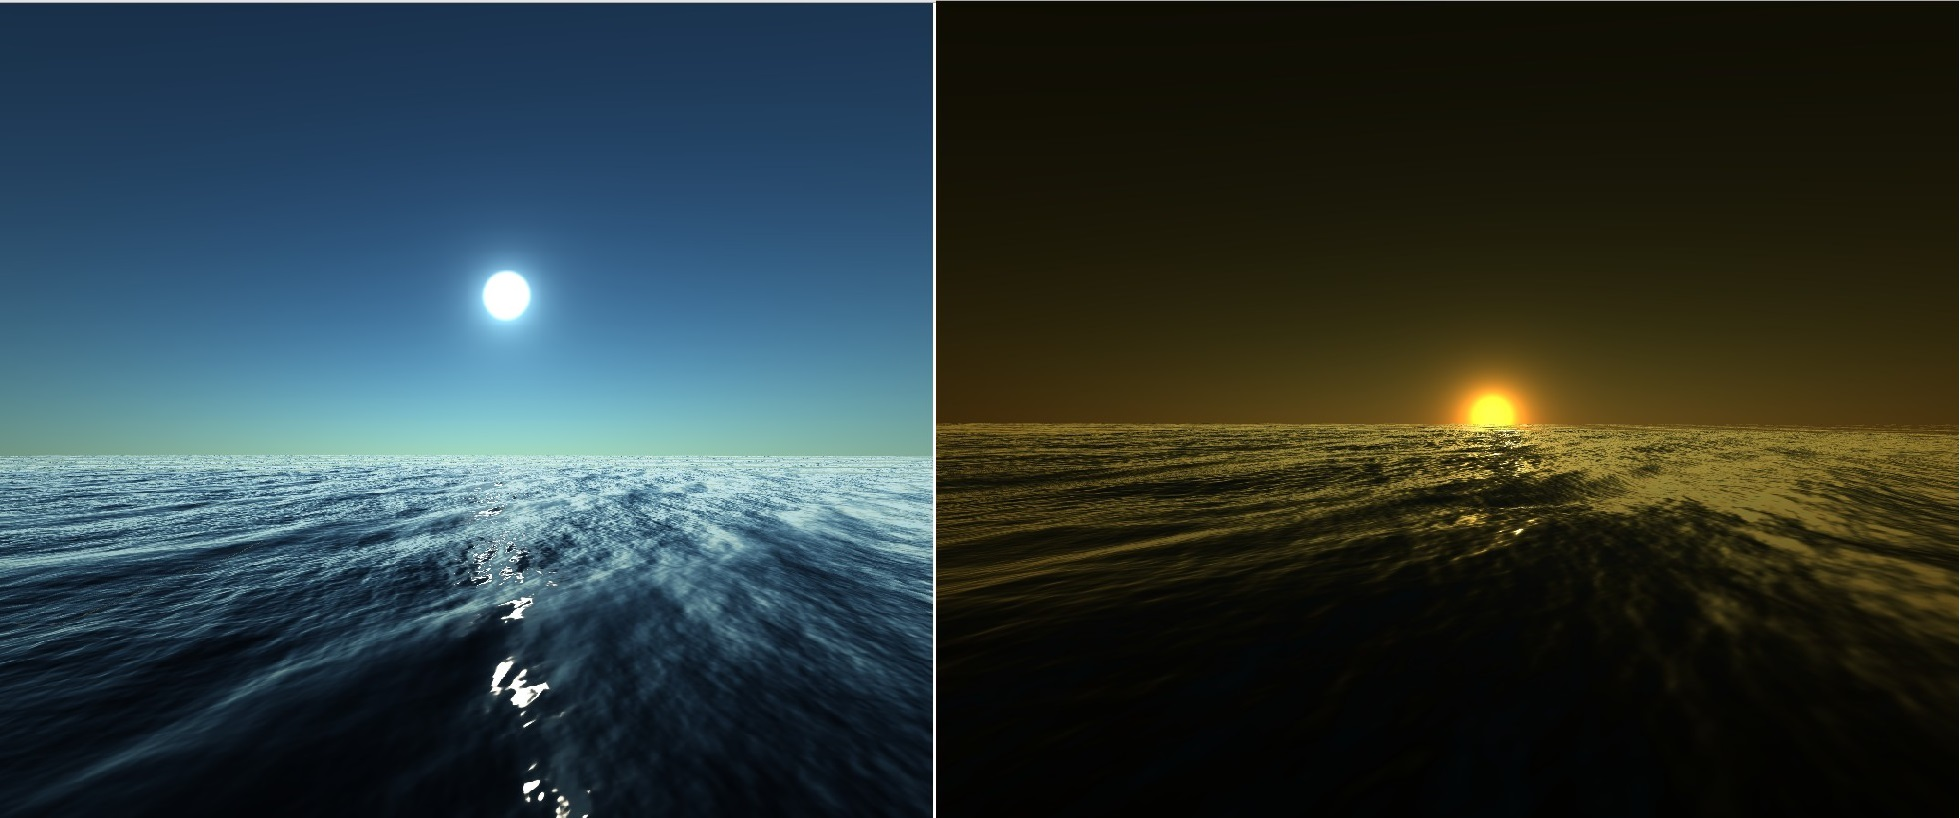
\includegraphics[width=5in]{frontpage.jpg}
  \label{fig:teaser}
}


\maketitle
\thispagestyle{firstpagestyle}

\begin{abstract}
FFT based height field based ocean simulation has been present in the industry for many years, and has become a sample program in many SDKs, such as CUDA and DirectX. However, in the area of WebGL,  there has not been a implementation that simulates ocean with FFT. We present an ocean simulation using custom FFT shader and discuss the rendering of the water surface as well as the physically based sky model.\\

Our implementation is capable of simulating and rendering visually infinite 512*512 tiled surface patches at 60 FPS on Core i7 processor and GTX TITAN. It has an simple GUI to adjust various simulation and rendering parameters on the fly. However, limited by the periodic nature of Discrete Fourier Transform, repeated pattern is visible viewed from a sufficiently high camera and seams between patches are difficult to remove entirely.
The Javascript and glsl code for this project is open source and available from our git repository.

\end{abstract}


%-------------------------------------------------------------------------
\section{Introduction}
\label{sec:introduction}
Our simulation and rendering pipeline consists of three major stages: simulation, (inverse) FFT, and rendering, shown in \ref{fig:pipeline}. Compared to the ocean simulation on HN\ref{enum:e2}, which generate a series of Gerstner Waves and superimpose to generate height field directly, we use statistical spectrum available from oceanography and do inverse FFT to obtain the height field. It is similar to the work done by Shiqiu(Edward) Liu\ref{enum:e1}, but on WebGL.

\begin{figure}[htb]
  \centering
   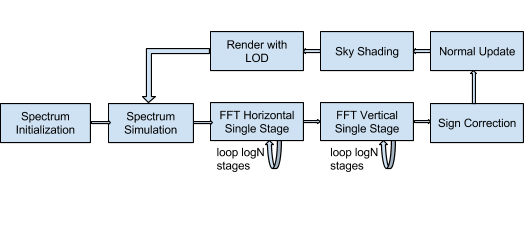
\includegraphics[width=0.8\textwidth]{pipeline.png}
   \caption{\label{fig:pipeline}
     The Pipeline of the WebGL ocean simulation and shading}
\end{figure}

\section{The Simulation and Rendering Pipeline}
\subsection{Build Statistical Wave Spectrum}
In our implementation, we reference Jerry Tessendorf's Simulating Ocean Water\ref{enum:e4} and model a patch of the ocean as a height field generated by Fast Fourier Transform from its statistical spectrum. The height field is represented as the inverse fourier transform:
\begin{equation}
h(\mathbf{x},t)=\sum_{\mathbf{k}} \tilde{h} (\mathbf{k},t) exp(i \mathbf{k} \cdot \mathbf{x})
\end{equation}
where t is time and $\mathbf{k}$ and $\mathbf{x}$ are grid points in frequency and spatial domain, respectively\\

Following the oceanographic research, for every grid points in the 2D frequency domain, Phillips Spectrum is computed as follows:
\begin{equation}
P_h (\mathbf{k})=A\frac{exp(-1/(kL)^2)}{k^4}|\hat{\mathbf{k}}\cdot\hat{w}| ^2
\end{equation}
where $L=V^2 /g$ and $V$ is the wind speed. $w$ is the wind direction. This result is then multiplied by $exp(-k^{2} l^{2})$ to suppress the very small waves which the macroscopic model no longer applies. In our implementation, $l=10^{-4}L$ \\

To generate the initial spectrum, we still need a gaussian number generator to generate two random numbers $\xi _r$ and $\xi _i$ and represent the spectrum at point $k$ as follows:
\begin{equation}
\tilde{h}_0 (\mathbf{k})=\frac{1}{\sqrt{2}}(\xi _r +i\xi _i )\sqrt{P_h  (\mathbf{k})}
\end{equation}

The gaussian number generator $\xi$ is implemented as a Box-Muller transform:
\begin{equation}
\xi = \sqrt{-2\ln{U_1}}\cos{(2\pi U_2)}
\end{equation}

where $U_1$ and $U_2$ are uniformly distributed random numbers in $[0, 1)$ and generated with Math.random(). Compute $\tilde{h}_0 (k)$ for every grid points in frequency domain and store the result in a floating point texture, which is enabled by OES\_texture\_float extension. The magnitude of $\tilde{h}_0 (k)$ is visualized in \ref{fig:h0k}

\begin{figure}[htb]
\begin{minipage}{0.49\textwidth}
\centering
   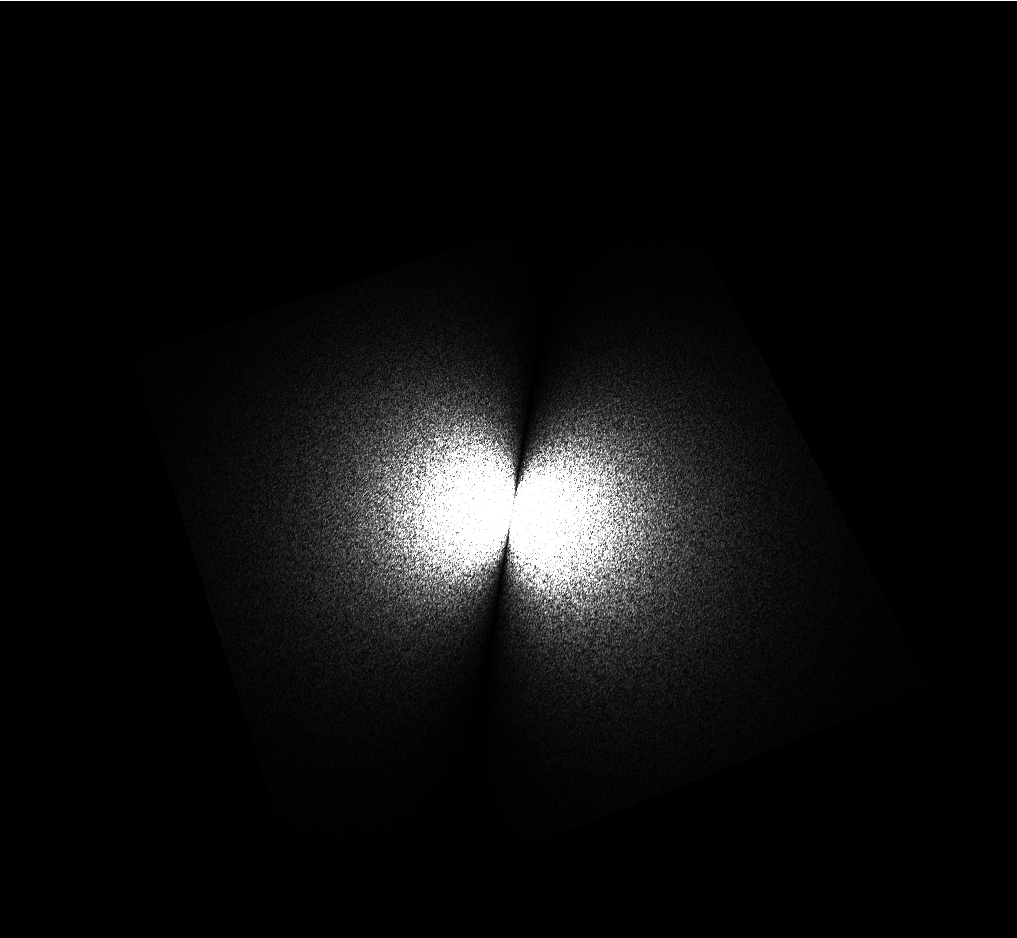
\includegraphics[height=5cm]{h0k.png}
   \caption{\label{fig:h0k}
      Magnitude of $\tilde{h}_0 (\mathbf{k})$}
\end{minipage}\hfill
\begin{minipage}{0.49\textwidth}
\centering
   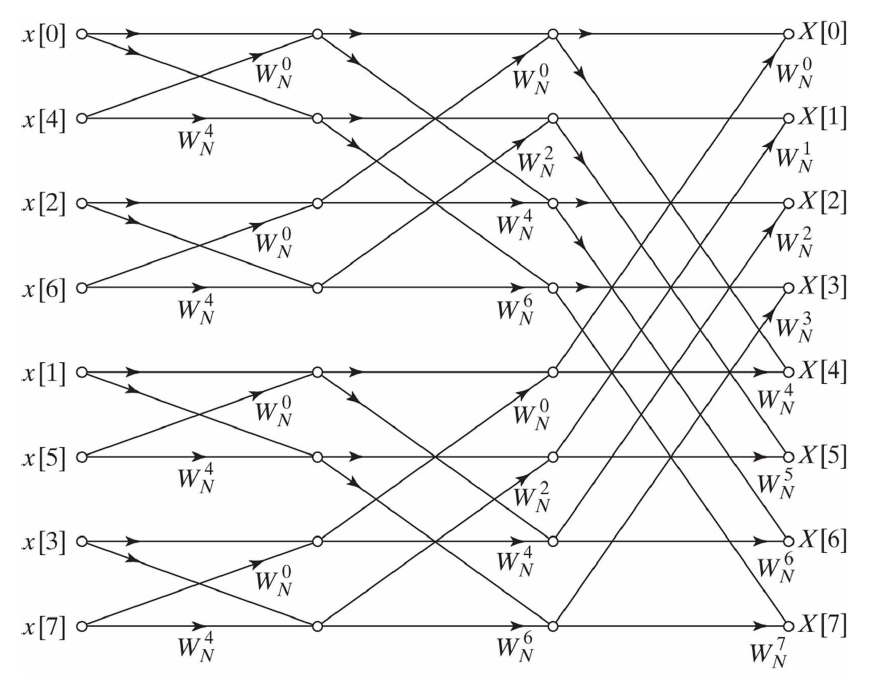
\includegraphics[height=5cm]{fft.png}
   \caption{\label{fig:fft}
      Illustration of FFT}
\end{minipage}\hfill
\end{figure}

\subsection{Fast Fourier Transform}

FFT is a computationally efficient algorithm to compute DFT and inverse DFT. The butterfly diagram is used when converting  data between frequency domain and space domain. See \ref{fig:fft}\\

In this 8-point case, the input data is first arranged in a bit-reversed order, and then, for each stage, with the help of precomputed weights and indices , each data point will retrieve its corresponding butterfly unit and calculate the data point used in the next stage of FFT. The weights and indices are stored in a texture for each stage and source data is stored in another texture. An intermediate texture is used in tandem with source texture to ping-pong between stages. \\

In our case, we perform 2D FFT instead of 1D. From the separability of FFT, a 2D FFT can be effectively decomposed to a 1D FFT for each row and a 1D FFT for each column of the result of the first 1D pass. The resulting texture now stores the height field in its real part. Note the above butterfly diagram is drawn for forward FFT. To use the same algorithm for inverse FFT, we simply use $W_N ^{-k}$ instead of $W_N ^k$ where $W_N \triangleq e^{-j2\pi / N}$\\

Before the height field data is actually usable, we need to invert the sign of every grid point where $x+y$ is even and $0 \leq x, y < N$. The theory behind this is still unknown to us, but it seems necessary from our experiment as well as the ocean FFT simulation from NVIDIA's CUDA sdk.\\

After sign correction and vertex normal calculation from nearby triangles' normal, the raw height image and normal's y component image are shown in \ref{fig:fftraw1} and \ref{fig:fftraw2}.
\begin{figure}[htb]
\begin{minipage}{0.49\textwidth}
\centering
   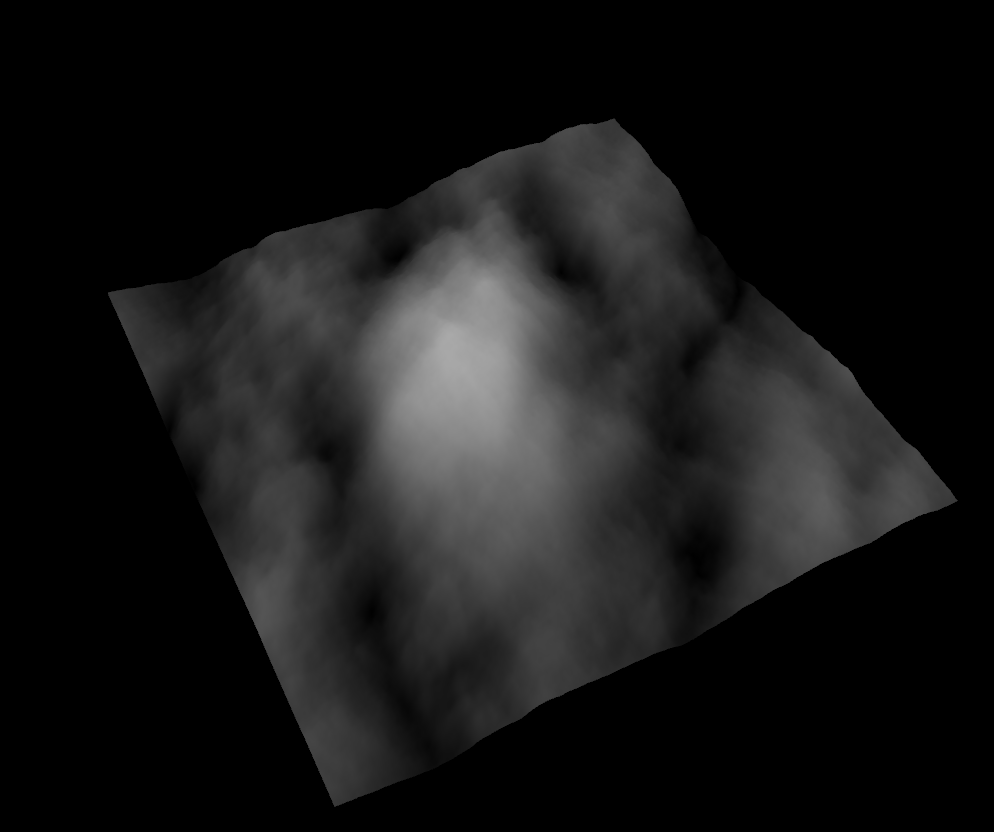
\includegraphics[height=5cm]{fft_raw1.png}
   \caption{\label{fig:fftraw1}
      Height map result}
\end{minipage}\hfill
\begin{minipage}{0.49\textwidth}
\centering
   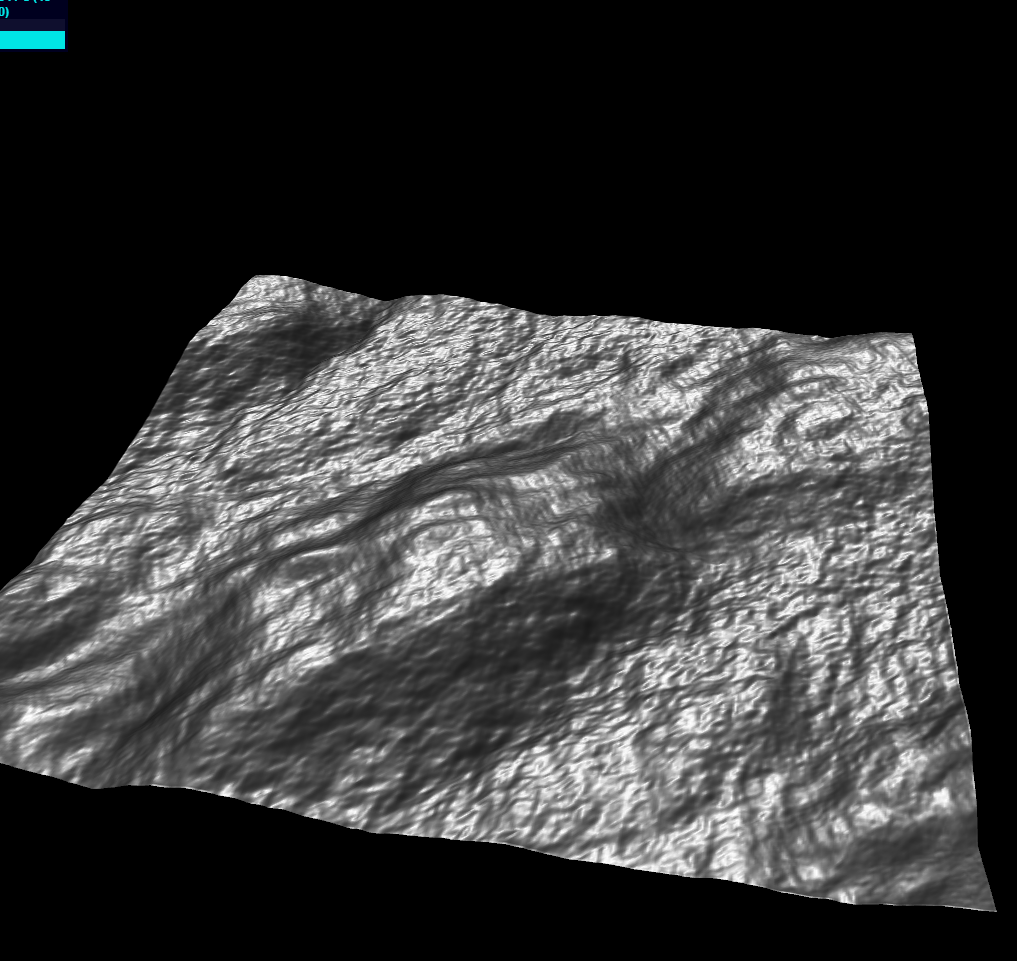
\includegraphics[height=5cm]{fft_raw2.png}
   \caption{\label{fig:fftraw2}
      Normal Map result}
\end{minipage}\hfill
\end{figure}

\subsection{Ocean Shading}
\subsubsection{Ocean Patch Shading}

An ocean patch is a piece of grid which has the same size as the height map from FFT step. The material of the ocean patch is considered as water material: reflection, refraction, no diffuse. The reflection rate is calculated by an approximated Fresnel equation:
\begin{equation}
\rho = \frac{1}{2} (\frac{\tan ^2 (\theta-\psi)}{\tan ^2 (\theta+\psi)} + \frac{\sin ^2 (\theta-\psi)}{\sin ^2 (\theta+\psi)} )
\end{equation}

where $\theta$ is the incident angle and $\psi$ is the refraction angle. The index of refraction of the water is $1.33$. \\

To calculate the normal of each grid point, the normal of the 4 triangles which shared this grid point are calculated and averaged to get the normal of the grid point.
With these normal and eye-ray information, the the fragment color is computed according to BRDF function:
\begin{equation}
 C_{output}=fresnel * C_{sky} + (1.0-fresnel) * C_{water} * C_{sky} * k_{skyAmbient}
\end{equation}
The skyColor is traced along the reflection direction. See \ref{sec:skyshading}.

\subsubsection{Infinite Ocean}

A key feature of an ocean is its infinity: one could barely travel out of an ocean. The most naive solution is drawing same patch multiple times with different position offset. The drawback of this method is its high cost: 262,144 vertices and 522,242 triangles per extra patch, with at least 100 extra patches required to make it looks "infinite". Unfortunately, cost is unacceptable for WebGL to keep it on a real-time level. \\

To settle this problem, we put forward a method similar to LOD: using low resolution grids for the patches far away from the eye, where the resolution is decided according to the distance from eye. We selected 3 levels of resolution: 128, 32 and 4. \\

Shading the low-resolution ocean is different from shading a full-resolution ocean in one part: the normal is calculated in fragment shader, rather than in vertex shader, with the same way. The shading effect looks generally the same with full-resolution ocean shading, if viewing from far away. See \ref{fig:lowres}

\begin{figure}[htb]
\centering
   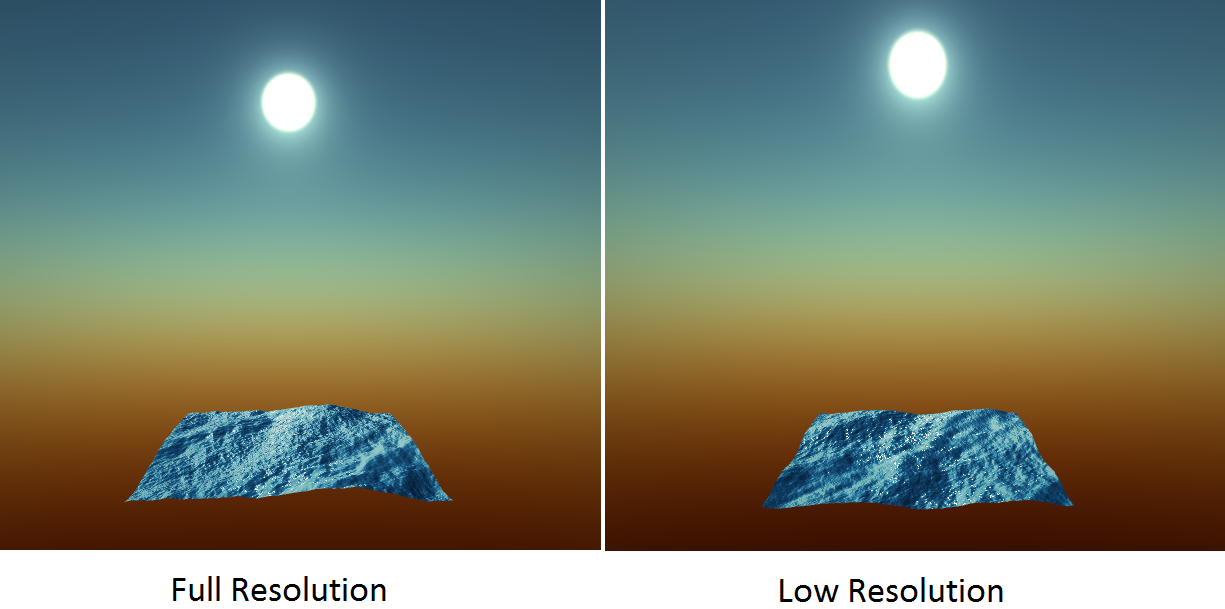
\includegraphics[width=0.8\textwidth]{lowres.png}
   \caption{\label{fig:lowres}
      Comparision between full resolution and low resolution result}

\end{figure}
\subsection{Sky Shading}
\label{sec:skyshading}
The sky shader simulates and renders the real sky. In the real world, there are countless tiny particles floating in the sky. The blue rays, with shorter wavelength, are more likely to be scattered by the particles, while the red rays are better at penetrating through particles. Obviously, the further a ray travels, the more likely it is scattered. \\

Based on the theory above, the sky shader is implemented with a ray-marching idea. The input is the viewing direction.
\begin{itemize}
\item[1.] March the position along the viewing direction
\item[2.] Calculate the distance from the sun
\item[3.] Accumulate the scattering of blue and red rays
\end{itemize}
The total scattering of blue and red rays is color of the sky.\\

For the viewing direction that pointing to the sun, however, (1.0-scatter) will be used instead, which indicated how much light has reach the eye. Then sum blue and red rays up to get the color of the sun.\\

Our implementation refer to the sky render from cloudpart.com\ref{enum:e3}. 

\section{Conclusion}
In our work, we present FFT ocean simulation, fresnel shading, sky simulation and shading, and LOD infinite ocean. This is the first realistic ocean view simulation and shading program on WebGL. \\

However, there are still many things need to be settled. First, with LOD method, we are drawing the same patch for hundreds of times. The regularity of the ocean surface is inevitable. When viewing from a high position, it looks unreal because of the regularity. Therefore, we are still seeking a solution for de-regularity. Second, there are actually some gaps between low resolution patches.\\

Our next steps contains adding fog effect and clouds in the scene. Fog effect may probably solve the problems above.

%\section{Source Code}
%\begin{lstlisting}[caption={A simple C program.}, label={lst:hello}, float]
%\end{lstlisting}

% \href{http://jcgt.org}{http://jcgt.org}.

%\section{Citations and Bibliography}
%Do not use citations as nouns--the text should read correctly were they omitted. For example, the following are correct:

%\begin{enumerate}
%\item ``The Rendering Equation \cite{Immel:1986:RMN:15886.15901,Kajiya:1986:RE:15922.15902} relates the incoming and outgoing light at a surface...''
%\item ``Immel et al.'s paper~\shortcite{Immel:1986:RMN:15886.15901} uses a directional parameterization...''
%\end{enumerate}

\small
\bibliographystyle{acmsiggraph}
\bibliography{paper}

\begin{enumerate}
\item \label{enum:e1} \href{http://www.edxgraphics.com/realistic-ocean-scene.html}{http://www.edxgraphics.com/realistic-ocean-scene.html}, Edward Liu
\item \label{enum:e2} \href{http://david.li/waves/}{http://david.li/waves/}, Ocean patch shader
\item \label{enum:e3} \href{https://www.cloudparty.com/studio/sky/ANdXh48Zy}{https://www.cloudparty.com/studio/sky/ANdXh48Zy}, Sky Render
\item \label{enum:e4} \textit{Simulating Ocean Water}, Jerry Tessendorf

\end{enumerate}
%\section*{Index of Supplemental Materials}
%When supplemental materials such as video, data sets, and source code are provided with an article, briefly describe them by directory or filename here.

%\section*{Author Contact Information}

%\hspace{-2mm}\begin{tabular}{p{0.5\textwidth}p{0.5\textwidth}}
%Roy G. Biv \newline
%Colortech, Inc. \newline
%29 Red Blvd. \newline
%New York, NY 10511 \newline
%\href{mailto:roy@colortech.com}{roy@colortech.com}
%&

%Raymond Trace \newline
%Graphica University \newline
%37 Rue De Lambert \newline
%Paris, 75009 France \newline
%\href{mailto:rtrace@graphica.edu}{rtrace@graphica.edu} \newline
%\href{http://graphica.edu/~rtrace}{http://graphica.edu/\textasciitilde rtrace}
%
%\end{tabular}


%\afterdoc

\end{document}
